\documentclass[12pt]{article}

% =============================================================================
% Paquetes y formato
% =============================================================================
\usepackage[utf8]{inputenc}
\usepackage[spanish,es-nodecimaldot]{babel}
\usepackage[margin=0.82in]{geometry}
\usepackage{amsmath,amsthm,amssymb,bm}
\usepackage{graphicx}
\usepackage{xcolor}
\definecolor{cideblue}{RGB}{5,35,75}
\definecolor{cidegray}{RGB}{80,85,92}

\graphicspath{{Figuras/Equilibrio_General/}}

\setlength{\parindent}{0pt}
\setlength{\parskip}{0.55em}
\allowdisplaybreaks

\pagestyle{plain}

\newtheoremstyle{cideplain}
  {0.8em}{0.8em}{\itshape}{}%
  {\bfseries\color{cideblue}}{.}{0.5em}{}
\newtheoremstyle{cidedef}
  {0.8em}{0.8em}{}{}%
  {\bfseries\color{cideblue}}{.}{0.5em}{}

\theoremstyle{cideplain}
\newtheorem{theorem}{Teorema}[section]
\newtheorem{proposition}[theorem]{Proposición}
\newtheorem{lemma}[theorem]{Lema}
\newtheorem{corollary}[theorem]{Corolario}

\theoremstyle{cidedef}
\newtheorem{definition}[theorem]{Definición}
\newtheorem{example}[theorem]{Ejemplo}
\newtheorem{remark}[theorem]{Observación}

\renewcommand{\proofname}{Demostración}
\DeclareMathOperator*{\argmax}{arg\,max}
\DeclareMathOperator{\MRS}{MRS}
\DeclareMathOperator{\MRT}{MRT}

\newcommand{\R}{\mathbb{R}}
\newcommand{\p}{\mathbf{p}}
\newcommand{\e}{\bm e}
\newcommand{\x}{\mathbf{x}}
\newcommand{\y}{\mathbf{y}}
\newcommand{\z}{\mathbf{z}}

% Referencias sin etiquetas cuadradas en la lista final.
\makeatletter
\renewenvironment{thebibliography}[1]
  {\section*{\refname}
   \list{}{\setlength{\leftmargin}{0pt}
           \setlength{\itemindent}{0pt}
           \setlength{\labelwidth}{0pt}
           \setlength{\labelsep}{0pt}
           \setlength{\itemsep}{0.7em}}
   \renewcommand\makelabel[1]{}
   \sloppy}
  {\endlist}
\makeatother

% =============================================================================
\begin{document}
% =============================================================================

\begin{center}
  {\large\bfseries Centro de Investigación y Docencia Económicas}\\[0.25em]
  {\large\bfseries Macroeconomía II --- Licenciatura en Economía}\\[0.8em]
  {\LARGE\bfseries\color{cideblue} Equilibrio general: intercambio y producción}\\[0.8em]
  {\large Handout de apoyo para el capítulo 5}\\[0.8em]
  Arturo López Pérez \hfill Otoño de 2026
\end{center}

\vspace{0.5em}
\hrule
\vspace{0.8em}

% =============================================================================
\section{De la decisión individual al equilibrio parcial}
% =============================================================================

En microeconomía, la teoría del consumidor es una \textit{teoría de la demanda}: dadas sus preferencias sobre una canasta de bienes y servicios, el vector de precios $\p$ y su ingreso $m$, el consumidor elige una canasta que maximiza su utilidad:

\[
\x(\p,m)
=
\arg\max_{\x\geq \bm 0}
\left\{
u(\x):
\p\cdot\x\leq m
\right\}.
\]

La solución de este problema se denomina \textit{demanda marshalliana}.
En general, se obtiene un vector de demandas
$\bm x(\bm p,m)=(x_1(\bm p,m),\ldots,x_L(\bm p,m))$, con una demanda para
cada bien. Si nos concentramos en el mercado del bien $i$, su demanda
puede escribirse como

\[
x_i^d(p_i;\bm p_{-i},m),
\]

donde $\bm p_{-i}$ contiene los precios de los demás bienes. Esta
expresión indica cuánto demanda el consumidor del bien $i$ para cada
valor de $p_i$, manteniendo constantes los demás precios y el ingreso.
Si la solución no es única, la demanda marshalliana es, formalmente, una
correspondencia y no necesariamente una función.

Por otro lado, la teoría del productor puede entenderse como una
\textit{teoría de la oferta}. Dada su tecnología y suponiendo que la
empresa es precio-aceptante, esta elige los insumos y la producción que
maximizan sus beneficios. En el caso de una empresa que produce el bien
$i$ mediante la tecnología $q_i=f(\bm v)$, su problema es

\[
\bm v^*(p_i,\bm r)
\in
\arg\max_{\bm v\geq\bm 0}
\left\{
p_i f(\bm v)-\bm r\cdot\bm v
\right\},
\]

donde $\bm r$ es el vector de precios de los insumos. La oferta
resultante es

\[
q_i^s(p_i,\bm r)
=
f\!\left(\bm v^*(p_i,\bm r)\right).
\]

Por tanto, para cada precio del producto y cada vector de precios de los
insumos, la función de oferta indica la cantidad que maximiza los
beneficios de la empresa. Al igual que la demanda, la oferta puede ser
una correspondencia cuando el problema tiene más de una solución.

La demanda total del mercado del bien $i$ es la suma de las demandas de
todos los consumidores, mientras que su oferta total es la suma de las
ofertas de todas las empresas:

\[
X_i^D(p_i;\bm p_{-i},\bm m)
=
\sum_h x_i^{d,h}(p_i;\bm p_{-i},m^h),
\qquad
X_i^S(p_i;\bm r)
=
\sum_j q_i^{s,j}(p_i,\bm r).
\]

Un \textit{equilibrio parcial} en el mercado del bien $i$ es un precio
$p_i^*$ y una cantidad $q_i^*$ tales que

\[
X_i^D(p_i^*;\bm p_{-i},\bm m)
=
q_i^*
=
X_i^S(p_i^*;\bm r),
\]

manteniendo constantes los precios de los demás bienes, los precios de
los insumos, los ingresos y los restantes parámetros. En este precio,
las decisiones óptimas de consumidores y empresas son compatibles: el
mercado se vacía.

En un \textit{equilibrio general}, en cambio, se determina un vector de
precios relativos $\bm p^*$ y una asignación tales que los consumidores
maximizan su utilidad, las empresas maximizan sus beneficios y todos los
mercados se vacían simultáneamente. En una economía con producción, esta
última condición puede escribirse como

\[
\sum_h \bm x^{h*}
=
\sum_h \bm e^h
+
\sum_j \bm y^{j*},
\]

donde $\bm e^h$ representa la dotación inicial del consumidor $h$ y
$\bm y^{j*}$ la producción neta de la empresa $j$. A diferencia del
análisis de equilibrio parcial, los precios, los ingresos y las
cantidades se determinan conjuntamente. Por ello, una perturbación
originada en un mercado puede modificar las decisiones y el equilibrio
de todos los demás mercados.

\subsection{Teoría del Consumidor}
Considere una economía con \(L\) bienes. Los consumidores están indexados por \(i\in\mathcal I=\{1,\ldots,I\}\). El consumidor \(i\) tiene preferencias representadas por una función de utilidad

\[
  u^i:\R_+^L\longrightarrow\R,
\]

que suponemos continua, localmente no saciable y cuasicóncava. Dados un vector de
precios \(\p\in\R_{++}^L\) y un ingreso monetario \(m^i>0\), su problema es

\begin{equation}
  \x^i(\p,m^i)
  \in
  \argmax_{\x^i\in\R_+^L}
  \left\{u^i(\x^i):\p\cdot\x^i\leq m^i\right\}.
  \label{eq:consumer-problem}
\end{equation}

\begin{definition}[Demanda marshalliana]
La correspondencia \(\x^i(\p,m^i)\) que resuelve \eqref{eq:consumer-problem} es la
\emph{demanda marshalliana} del consumidor \(i\). Si la solución es única, es una función.
Su componente \(\ell\), denotada \(x_\ell^i(\p,m^i)\), indica cuánto demanda del bien
\(\ell\) a cada vector de precios e ingreso.
\end{definition}

La teoría del consumidor produce, por tanto, un \emph{sistema} de demandas: una demanda
para cada bien y no solamente una curva aislada. Si estudiamos el mercado del bien 1,
la demanda total es la suma de las demandas individuales:

\begin{equation}
  X_1^D(p_1;\p_{-1},\bm m)
  =\sum_{i\in\mathcal I}x_1^i(p_1,\p_{-1},m^i),
  \label{eq:market-demand}
\end{equation}

donde \(\p_{-1}\) contiene los precios de todos los bienes distintos del bien 1 y
\(\bm m=(m^1,\ldots,m^I)\). Una curva de demanda parcial mantiene fijos
\(\p_{-1}\) y \(\bm m\) mientras varía \(p_1\).

\subsection{La teoría del productor como teoría de la oferta}

Las empresas están indexadas por \(j\in\mathcal J=\{1,\ldots,J\}\). Para comenzar,
suponga que la empresa \(j\) produce el bien 1 mediante la tecnología

\[
  q_1^j\leq f^j(\bm v^j),
\]

donde \(\bm v^j\in\R_+^K\) es un vector de insumos y \(\bm r\in\R_{++}^K\) contiene
sus precios. Si la empresa es precio-aceptante, elige insumos para maximizar beneficios:

\begin{equation}
  \bm v^{j*}(p_1,\bm r)
  \in
  \argmax_{\bm v^j\geq\bm 0}
  \left\{p_1f^j(\bm v^j)-\bm r\cdot\bm v^j\right\}.
  \label{eq:firm-problem-partial}
\end{equation}

La oferta de la empresa es

\[
  q_1^{j,S}(p_1,\bm r)=f^j\!\left(\bm v^{j*}(p_1,\bm r)\right),
\]

y la oferta total del mercado es

\begin{equation}
  X_1^S(p_1;\bm r)=\sum_{j\in\mathcal J}q_1^{j,S}(p_1,\bm r).
  \label{eq:market-supply}
\end{equation}

En una formulación de varios bienes, cada empresa posee un conjunto de producción
\(Y^j\subseteq\R^L\) y elige un vector de producción neta

\[
  \y^j(\p)\in\argmax_{\y\in Y^j}\p\cdot\y.
\]

Las componentes positivas de \(\y^j\) son productos y las negativas son insumos. Esta
notación será útil cuando estudiemos equilibrio general con producción.

\subsection{Equilibrio en el mercado de un solo bien}

\begin{definition}[Equilibrio parcial]
Dados \(\p_{-1}\), los ingresos \(\bm m\), los precios de los insumos \(\bm r\), las
preferencias, las tecnologías y los demás parámetros, un equilibrio parcial en el mercado
del bien 1 es un precio \(p_1^*>0\) y una cantidad \(Q_1^*\) tales que

\begin{equation}
  X_1^D(p_1^*;\p_{-1},\bm m)
  =Q_1^*
  =X_1^S(p_1^*;\bm r).
  \label{eq:partial-equilibrium}
\end{equation}
\end{definition}

En \(p_1^*\), cada consumidor elige una canasta que maximiza su utilidad, cada empresa
elige una producción que maximiza sus beneficios y las decisiones agregadas son
compatibles en el mercado del bien 1. Se dice que el mercado \emph{se vacía}.

El calificativo \emph{parcial} es esencial: los precios de otros bienes, los ingresos y los
precios de los insumos se tratan como datos. Un cambio en este mercado no retroalimenta,
dentro del análisis, los demás mercados.

\begin{remark}[Agentes representativos]
Si existe una unidad de masa de consumidores y empresas idénticos, podemos normalizar
su masa a uno. Bajo esa normalización, la demanda y la oferta del agente representativo
coinciden con sus contrapartes agregadas. Así, la condición de equilibrio parcial se reduce a

\[
  x_1^R(p_1^*;\cdot)=q_1^R(p_1^*;\cdot).
\]

Sin esta normalización, la demanda u oferta individual debe multiplicarse por el número o
la masa de agentes. El agente representativo debe interpretarse como una representación
de los agregados, no como la afirmación de que sólo existe una persona o una empresa.
\end{remark}

\begin{example}[Demanda y oferta lineales]
Si \(X_1^D(p_1)=a-bp_1\) y \(X_1^S(p_1)=c+dp_1\), con \(b,d>0\) y \(a>c\), entonces

\[
  p_1^*=\frac{a-c}{b+d},
  \qquad
  Q_1^*=\frac{ad+bc}{b+d}.
\]

Estos valores dependen de los parámetros \(a,b,c,d\), que resumen las variables mantenidas
constantes. Si, por ejemplo, el ingreso modifica \(a\), la curva de demanda se desplaza y el
equilibrio parcial cambia.
\end{example}

% =============================================================================
\section{Equilibrio general: intercambio puro}
% =============================================================================

\subsection{La economía y sus asignaciones factibles}

Considere dos bienes, \(1\) y \(2\), y dos agentes, \(A\) y \(B\). No existe producción:
los bienes disponibles provienen de las dotaciones iniciales. La economía se describe por

\[
  \mathcal E=
  \left\{u^A,u^B,\e^A,\e^B\right\},
\]

donde

\[
  \e^A=(e_1^A,e_2^A),
  \qquad
  \e^B=(e_1^B,e_2^B),
\]

y la dotación agregada es

\[
  \overline{\e}=\e^A+\e^B
  =(\overline e_1,\overline e_2)\gg\bm 0.
\]

Una asignación es un par \((\x^A,\x^B)\). Es factible si

\begin{equation}
  \x^A+\x^B\leq\overline{\e}.
  \label{eq:feasibility-exchange}
\end{equation}

Con preferencias localmente no saciables, ninguna asignación eficiente desperdicia bienes,
por lo que \eqref{eq:feasibility-exchange} se cumple con igualdad.

\begin{figure}[htbp]
  \centering
  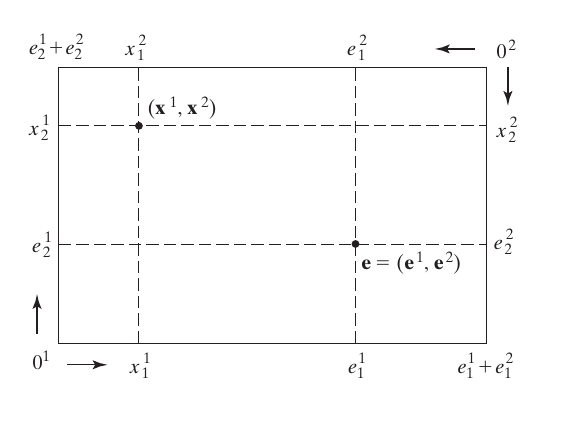
\includegraphics[width=0.72\textwidth]{edgeworth_caja.png}
  \caption{Caja de Edgeworth para dos bienes y dos agentes. Cada punto representa una
  asignación factible; las cantidades de \(A\) se miden desde el origen suroeste y las de
  \(B\) desde el noreste. Los agentes 1 y 2 de la figura corresponden a \(A\) y \(B\),
  respectivamente. Fuente: (Jehle y Reny, 2011, fig. 5.1).}
  \label{fig:edgeworth-basic}
\end{figure}
\clearpage

La caja tiene ancho \(\overline e_1\) y altura \(\overline e_2\). Una vez elegida la canasta
de \(A\), la canasta de \(B\) está determinada por factibilidad:

\[
  \x^B=\overline{\e}-\x^A.
\]

Por ello, un solo punto de la caja proporciona las cuatro cantidades
\((x_1^A,x_2^A,x_1^B,x_2^B)\).

\subsection{Eficiencia de Pareto y la curva de contrato}

\begin{definition}[Mejora de Pareto]
Una asignación factible \((\widehat{\x}^A,\widehat{\x}^B)\) es una mejora de Pareto
respecto de \((\x^A,\x^B)\) si

\[
  u^i(\widehat{\x}^i)\geq u^i(\x^i),
  \qquad i\in\{A,B\},
\]

y al menos una de las dos desigualdades es estricta.
\end{definition}

\begin{definition}[Asignación eficiente en el sentido de Pareto]
Una asignación factible \((\x^A,\x^B)\) es eficiente en el sentido de Pareto si no existe
otra asignación factible que constituya una mejora de Pareto.
\end{definition}

En el interior de la caja, suponga que las utilidades son diferenciables, estrictamente
crecientes y estrictamente cuasicóncavas. La tasa marginal de sustitución del bien 1 por el
bien 2 para el agente \(i\) es

\[
  \MRS_{12}^i(\x^i)
  =\frac{\partial u^i(\x^i)/\partial x_1^i}
         {\partial u^i(\x^i)/\partial x_2^i}.
\]

\begin{proposition}[Condición interior de eficiencia]
Si una asignación interior es eficiente en el sentido de Pareto, entonces

\begin{equation}
  \MRS_{12}^A(\x^A)=\MRS_{12}^B(\x^B).
  \label{eq:mrs-efficiency}
\end{equation}
\end{proposition}

\begin{proof}
Si las tasas marginales de sustitución fueran distintas, existiría una dirección de
intercambio suficientemente pequeña que aumentaría el bienestar de ambos agentes. Por
ejemplo, si \(\MRS_{12}^A>\MRS_{12}^B\), el agente \(A\) estaría dispuesto a entregar más
del bien 2 por una unidad del bien 1 de lo que exigiría \(B\) para entregar esa unidad.
Un intercambio a una tasa estrictamente intermedia mejoraría a ambos, contradiciendo la
eficiencia de la asignación inicial.
\end{proof}

El conjunto de asignaciones eficientes forma la \emph{curva de contrato}. También puede
obtenerse resolviendo, para cada peso social \(\lambda\in(0,1)\),

\begin{equation}
  \max_{\x^A,\x^B}
  \lambda u^A(\x^A)+(1-\lambda)u^B(\x^B)
  \quad\text{sujeto a}\quad
  \x^A+\x^B=\overline{\e}.
  \label{eq:planner-exchange}
\end{equation}

Variar \(\lambda\) recorre las distintas asignaciones eficientes y deja claro que eficiencia
no equivale a igualdad distributiva.

\begin{figure}[htbp]
  \centering
  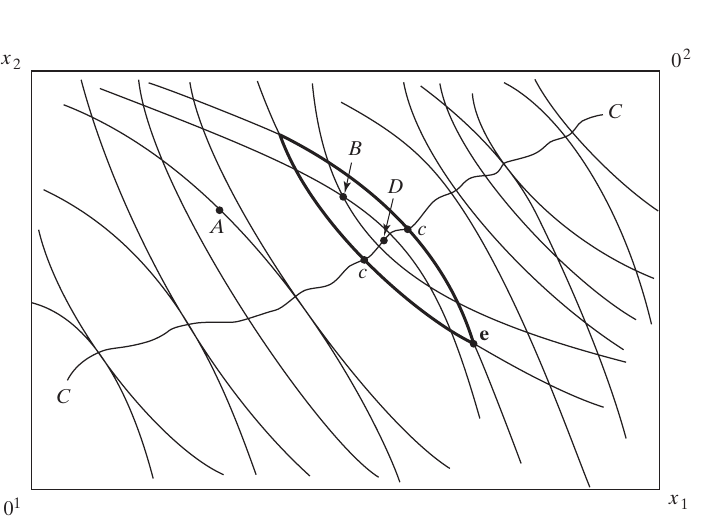
\includegraphics[width=0.78\textwidth]{edgeworth_contrato.png}
  \caption{Curvas de indiferencia, curva de contrato \(C\) y conjunto de asignaciones que
  permiten ganancias de intercambio respecto de la dotación inicial. Los agentes 1 y 2 de
  la figura corresponden a \(A\) y \(B\). Fuente: (Jehle y Reny, 2011, fig. 5.2).}
  \label{fig:edgeworth-contract}
\end{figure}
\clearpage

\subsection{Equilibrio walrasiano}

Sea \(\p=(p_1,p_2)\gg\bm 0\) el vector de precios. En una economía de intercambio puro,
el valor de la dotación inicial determina el ingreso de cada agente:

\[
  m^i(\p)=\p\cdot\e^i,
  \qquad i\in\{A,B\}.
\]

Cada agente resuelve

\begin{equation}
  \x^i(\p)
  \in
  \argmax_{\x^i\geq\bm 0}
  \left\{u^i(\x^i):\p\cdot\x^i\leq\p\cdot\e^i\right\}.
  \label{eq:consumer-exchange}
\end{equation}

Observe una diferencia central respecto del equilibrio parcial: el ingreso ya no es una
constante externa. Depende de los precios de equilibrio a través del valor de la dotación.

\begin{definition}[Equilibrio walrasiano]
Un equilibrio walrasiano es un vector de precios \(\p^*\gg\bm 0\) y una asignación
\((\x^{A*},\x^{B*})\) tales que:

\begin{enumerate}
  \item para cada \(i\in\{A,B\}\), \(\x^{i*}\) resuelve
  \eqref{eq:consumer-exchange} a precios \(\p^*\);
  \item todos los mercados se vacían:
  \begin{equation}
    \x^{A*}+\x^{B*}=\overline{\e}.
    \label{eq:market-clearing-exchange}
  \end{equation}
\end{enumerate}
\end{definition}

Defina la demanda excedente agregada

\[
  \z(\p)
  =\x^A(\p)+\x^B(\p)-\overline{\e}.
\]

Entonces \(\p^*\) es un vector de precios de equilibrio si

\[
  \z(\p^*)=\bm 0.
\]

\begin{proposition}[Ley de Walras]
Si las preferencias son localmente no saciables, la demanda excedente satisface

\begin{equation}
  \p\cdot\z(\p)=0
  \label{eq:walras-law}
\end{equation}

para todo \(\p\gg\bm 0\).
\end{proposition}

\begin{proof}
La no saciedad local implica que cada restricción presupuestaria se cumple con igualdad:
\(\p\cdot\x^i(\p)=\p\cdot\e^i\). Sumando sobre \(i=A,B\),

\[
  \p\cdot\left[\x^A(\p)+\x^B(\p)-\e^A-\e^B\right]=0,
\]

que es exactamente \eqref{eq:walras-law}.
\end{proof}

En una economía de dos bienes, \(p_1z_1(\p)+p_2z_2(\p)=0\). Por tanto, si un mercado
se vacía, el otro también. Además, las demandas son homogéneas de grado cero en precios:
sólo importa el precio relativo. Podemos normalizar \(p_2=1\) y buscar

\[
  q^*=\frac{p_1^*}{p_2^*}
  \quad\text{tal que}\quad
  z_1(q^*,1)=0.
\]

\begin{figure}[htbp]
  \centering
  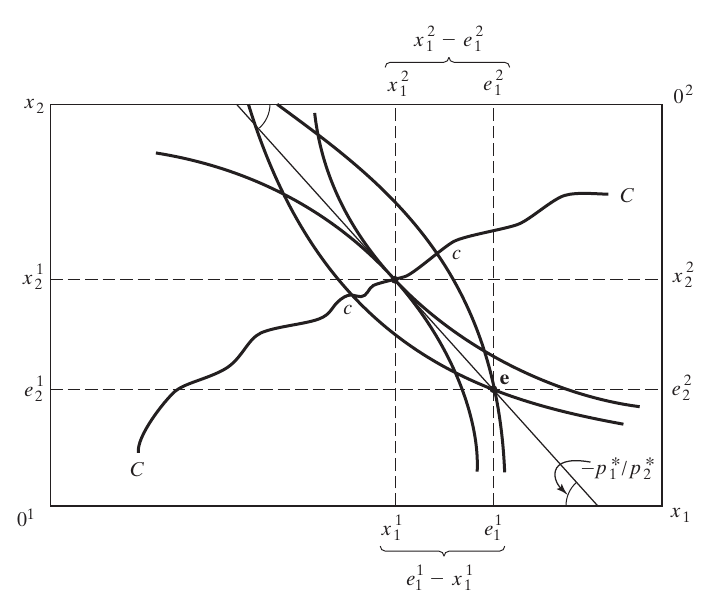
\includegraphics[width=0.78\textwidth]{edgeworth_walras.png}
  \caption{Equilibrio walrasiano en la caja de Edgeworth. La recta presupuestaria común
  pasa por la dotación inicial y su pendiente es \(-p_1^*/p_2^*\). Los agentes 1 y 2 de
  la figura corresponden a \(A\) y \(B\). Fuente: (Jehle y Reny, 2011, fig. 5.4).}
  \label{fig:edgeworth-walras}
\end{figure}
\clearpage

\subsection{Un equilibrio walrasiano resuelto}

Suponga preferencias Cobb--Douglas:

\[
  u^A(\x^A)=(x_1^A)^\alpha(x_2^A)^{1-\alpha},
  \qquad
  u^B(\x^B)=(x_1^B)^\beta(x_2^B)^{1-\beta},
\]

con \(0<\alpha,\beta<1\). Normalice \(p_2=1\) y denote \(q=p_1/p_2=p_1\). La riqueza
de cada agente es

\[
  m^A(q)=qe_1^A+e_2^A,
  \qquad
  m^B(q)=qe_1^B+e_2^B.
\]

Las demandas marshallianas son

\begin{align*}
  x_1^A(q)&=\alpha\frac{m^A(q)}{q},
  &x_2^A(q)&=(1-\alpha)m^A(q),\\
  x_1^B(q)&=\beta\frac{m^B(q)}{q},
  &x_2^B(q)&=(1-\beta)m^B(q).
\end{align*}

El vaciamiento del mercado del bien 1 requiere

\[
  \alpha e_1^A+\beta e_1^B
  +\frac{\alpha e_2^A+\beta e_2^B}{q}
  =e_1^A+e_1^B.
\]

Por tanto, el precio relativo de equilibrio es

\begin{equation}
  q^*
  =\frac{p_1^*}{p_2^*}
  =\frac{\alpha e_2^A+\beta e_2^B}
  {(1-\alpha)e_1^A+(1-\beta)e_1^B}.
  \label{eq:cobb-douglas-price}
\end{equation}

La ley de Walras garantiza que, al sustituir \(q^*\), también se vacía el mercado del bien
2. Las cantidades de equilibrio se obtienen evaluando las demandas en \(q^*\).

\begin{example}[Dotaciones especializadas]
Sea \(\alpha=\beta=1/2\), \(\e^A=(1,0)\) y \(\e^B=(0,1)\). De
\eqref{eq:cobb-douglas-price},

\[
  \frac{p_1^*}{p_2^*}=1.
\]

Cada agente tiene riqueza igual a uno y demanda

\[
  \x^{A*}=\x^{B*}=\left(\frac12,\frac12\right).
\]

El agente \(A\) entrega media unidad del bien 1 a cambio de media unidad del bien 2; el
agente \(B\) realiza el intercambio opuesto. Ambos mercados se vacían simultáneamente.
\end{example}

\subsection{El primer teorema del bienestar}

\begin{theorem}[Primer teorema fundamental del bienestar]
Suponga que las preferencias de ambos agentes son localmente no saciables y que
\(\p^*\gg\bm 0\). Toda asignación de equilibrio walrasiano es eficiente en el sentido de
Pareto.
\end{theorem}

\begin{proof}
Sea \((\p^*,\x^{A*},\x^{B*})\) un equilibrio walrasiano. Suponga, buscando una
contradicción, que su asignación no es eficiente. Entonces existe una asignación factible
\((\widehat{\x}^A,\widehat{\x}^B)\) tal que

\[
  u^i(\widehat{\x}^i)\geq u^i(\x^{i*}),
  \qquad i\in\{A,B\},
\]

con una desigualdad estricta para al menos un agente.

Por optimalidad individual y no saciedad local, cualquier canasta débilmente preferida a
\(\x^{i*}\) debe costar al menos la riqueza del agente:

\[
  \p^*\cdot\widehat{\x}^i
  \geq \p^*\cdot\e^i.
\]

Para el agente que mejora estrictamente, la desigualdad debe ser estricta; de otro modo,
la canasta alternativa habría sido asequible y contradiría la optimalidad de \(\x^{i*}\).
Sumando sobre los dos agentes,

\begin{equation}
  \p^*\cdot
  \left(\widehat{\x}^A+\widehat{\x}^B\right)
  >
  \p^*\cdot\left(\e^A+\e^B\right).
  \label{eq:welfare-expensive}
\end{equation}

Sin embargo, la factibilidad de la asignación alternativa implica

\[
  \widehat{\x}^A+\widehat{\x}^B
  \leq\e^A+\e^B.
\]

Como \(\p^*\gg\bm 0\), esta desigualdad contradice
\eqref{eq:welfare-expensive}. Por tanto, la asignación walrasiana es eficiente en el
sentido de Pareto.
\end{proof}

En una solución interior y diferenciable, la optimalidad de cada consumidor implica

\[
  \MRS_{12}^A(\x^{A*})
  =\frac{p_1^*}{p_2^*}
  =\MRS_{12}^B(\x^{B*}).
\]

Así, el equilibrio se encuentra sobre la curva de contrato. El precio relativo común
coordina decisiones descentralizadas y elimina oportunidades de intercambio mutuamente
beneficioso.

\begin{remark}[Segundo teorema del bienestar]
Bajo preferencias continuas, convexas y localmente no saciables, una asignación eficiente
puede descentralizarse mediante precios competitivos después de una redistribución
apropiada de la riqueza inicial. El primer teorema separa eficiencia y distribución: un
equilibrio competitivo puede ser eficiente sin ser considerado equitativo. El segundo
teorema indica, bajo condiciones adicionales, que la distribución puede modificarse con
transferencias de suma fija antes de permitir el intercambio competitivo; véase Jehle y
Reny (2011, cap. 5).
\end{remark}

% =============================================================================
\section{Equilibrio general con producción}
% =============================================================================

\subsection{Empresas, propiedad y riqueza}

Regrese a una economía con \(L\) bienes, \(I\) consumidores y \(J\) empresas. Cada
empresa \(j\) tiene un conjunto de producción \(Y^j\subseteq\R^L\) y elige un plan de
producción neta resolviendo

\begin{equation}
  \y^{j}(\p)
  \in\argmax_{\y\in Y^j}\p\cdot\y,
  \qquad
  \pi^j(\p)=\p\cdot\y^j(\p).
  \label{eq:profit-general}
\end{equation}

Sea \(\theta_{ij}\in[0,1]\) la participación del consumidor \(i\) en la empresa \(j\), con

\[
  \sum_{i=1}^I\theta_{ij}=1
  \qquad\text{para cada }j.
\]

La riqueza del consumidor \(i\) incluye el valor de su dotación y su participación en los
beneficios:

\begin{equation}
  m^i(\p)
  =\p\cdot\e^i
  +\sum_{j=1}^J\theta_{ij}\pi^j(\p).
  \label{eq:wealth-production}
\end{equation}

Su demanda se obtiene de

\begin{equation}
  \x^i(\p)
  \in\argmax_{\x\geq\bm 0}
  \left\{u^i(\x):\p\cdot\x\leq m^i(\p)\right\}.
  \label{eq:consumer-production}
\end{equation}

\subsection{Definición del equilibrio}

\begin{definition}[Equilibrio walrasiano con producción]
Un vector de precios \(\p^*\gg\bm 0\), una asignación de consumo
\((\x^{1*},\ldots,\x^{I*})\) y planes de producción
\((\y^{1*},\ldots,\y^{J*})\) constituyen un equilibrio walrasiano si:

\begin{enumerate}
  \item cada consumidor resuelve \eqref{eq:consumer-production} a precios \(\p^*\);
  \item cada empresa resuelve \eqref{eq:profit-general} a precios \(\p^*\);
  \item todos los mercados se vacían:
  \begin{equation}
    \sum_{i=1}^I\x^{i*}
    =\sum_{i=1}^I\e^i+\sum_{j=1}^J\y^{j*}.
    \label{eq:market-clearing-production}
  \end{equation}
\end{enumerate}
\end{definition}

La ecuación \eqref{eq:market-clearing-production} tiene una componente por bien. Los
recursos consumidos no pueden exceder las dotaciones más la producción neta. Los precios
son nuevamente relativos: si las decisiones son homogéneas de grado cero, una
normalización elimina un grado de libertad.

\subsection{Eficiencia con producción}

\begin{definition}[Factibilidad con producción]
Una asignación \((\x,\y)\) es factible si \(\y^j\in Y^j\) para cada empresa y

\[
  \sum_{i=1}^I\x^i
  \leq\sum_{i=1}^I\e^i+\sum_{j=1}^J\y^j.
\]
\end{definition}

\begin{theorem}[Primer teorema del bienestar con producción]
Si las preferencias son localmente no saciables, toda asignación de equilibrio walrasiano
con producción es eficiente en el sentido de Pareto.
\end{theorem}

\begin{proof}
Suponga que existe una asignación factible alternativa
\((\widehat{\x},\widehat{\y})\) que mejora débilmente a todos los consumidores y
estrictamente a uno. Por optimalidad individual,

\[
  \p^*\cdot\widehat{\x}^i\geq m^i(\p^*)
\]

para todo \(i\), con desigualdad estricta para al menos uno. Sumando y usando que las
participaciones de propiedad suman uno,

\begin{equation}
  \p^*\cdot\sum_i\widehat{\x}^i
  >
  \p^*\cdot\sum_i\e^i+\sum_j\pi^j(\p^*).
  \label{eq:production-expensive}
\end{equation}

Por factibilidad,

\[
  \p^*\cdot\sum_i\widehat{\x}^i
  \leq
  \p^*\cdot\sum_i\e^i
  +\sum_j\p^*\cdot\widehat{\y}^j.
\]

La maximización de beneficios implica

\[
  \p^*\cdot\widehat{\y}^j
  \leq\p^*\cdot\y^{j*}
  =\pi^j(\p^*)
\]

para cada \(j\). Estas dos desigualdades contradicen
\eqref{eq:production-expensive}. Por tanto, no existe una mejora de Pareto factible.
\end{proof}

% =============================================================================
\section{Williamson: el modelo macroeconómico de un periodo}
% =============================================================================

El capítulo 5 de Williamson (2018) especializa la estructura anterior a una economía
cerrada de un periodo con un consumidor representativo, una empresa representativa, un
bien de consumo y trabajo. El capital \(K\), la productividad total de los factores \(z\) y
el gasto público \(G\) son exógenos.

\subsection{Problemas individuales}

El consumidor representativo elige consumo \(C\) y oferta laboral \(N^s\), o de manera
equivalente ocio \(\ell=\bar h-N^s\), para resolver

\begin{equation}
  \max_{C,N^s}\ U(C,\bar h-N^s)
  \quad\text{sujeto a}\quad
  C=wN^s+\Pi-T,
  \label{eq:williamson-consumer}
\end{equation}

donde \(w\) es el salario real, \(\Pi\) son los beneficios distribuidos por la empresa y
\(T\) son impuestos de suma fija. En una solución interior,

\begin{equation}
  \MRS_{\ell,C}=w.
  \label{eq:williamson-consumer-foc}
\end{equation}

La empresa representativa elige demanda de trabajo \(N^d\):

\begin{equation}
  \max_{N^d\geq0}
  \Pi=zF(K,N^d)-wN^d.
  \label{eq:williamson-firm}
\end{equation}

La condición interior de maximización de beneficios es

\begin{equation}
  zF_N(K,N^d)=\mathrm{MPN}=w.
  \label{eq:williamson-firm-foc}
\end{equation}

Finalmente, el gobierno satisface una restricción presupuestaria balanceada:

\begin{equation}
  T=G.
  \label{eq:government-budget}
\end{equation}

\subsection{Condiciones de equilibrio}

Un equilibrio competitivo es un salario real \(w^*\) y cantidades
\((C^*,N^{s*},N^{d*},Y^*,T^*,\Pi^*)\) tales que los agentes optimizan y

\begin{align}
  N^{s*}&=N^{d*}=N^*,
  &&\text{vaciamiento del mercado de trabajo},
  \label{eq:labor-clearing}\\
  Y^*&=zF(K,N^*),
  &&\text{producción agregada},
  \label{eq:output}\\
  \Pi^*&=Y^*-w^*N^*,
  &&\text{beneficios distribuidos},
  \label{eq:profits}\\
  T^*&=G,
  &&\text{presupuesto del gobierno},
  \label{eq:government}\\
  Y^*&=C^*+G,
  &&\text{vaciamiento del mercado de bienes}.
  \label{eq:goods-clearing}
\end{align}

La última ecuación no es independiente. Sustituyendo
\(\Pi^*=Y^*-w^*N^{d*}\), \(T^*=G\) y \(N^{s*}=N^{d*}\) en la restricción
presupuestaria del consumidor se obtiene \(C^*=Y^*-G\). Ésta es la manifestación de la
ley de Walras en el modelo: una vez que optimización, presupuestos y el mercado de trabajo
son consistentes, el mercado de bienes también se vacía.

\subsection{La condición de eficiencia}

Combinando \eqref{eq:williamson-consumer-foc} y
\eqref{eq:williamson-firm-foc},

\begin{equation}
  \MRS_{\ell,C}=w^*=\mathrm{MPN}=\MRT_{\ell,C}.
  \label{eq:macro-efficiency}
\end{equation}

El salario real es el precio relativo que coordina al consumidor y a la empresa. Para el
consumidor, mide el costo de oportunidad del ocio; para la empresa, mide el costo de una
unidad adicional de trabajo. En equilibrio, la valoración marginal del ocio en términos de
consumo coincide con la cantidad de consumo que tecnológicamente puede obtenerse al
renunciar a una unidad de ocio.

Un planificador social resolvería

\begin{equation}
  \max_{C,N}\ U(C,\bar h-N)
  \quad\text{sujeto a}\quad
  C+G\leq zF(K,N).
  \label{eq:social-planner-macro}
\end{equation}

Su condición interior es exactamente \eqref{eq:macro-efficiency}. Por ello, bajo
competencia perfecta, ausencia de externalidades e impuestos no distorsionantes, la
asignación competitiva coincide con la asignación eficiente del planificador. Ésta es la
versión macroeconómica del primer teorema del bienestar.

Los ejercicios de estática comparativa del capítulo 5 ---cambios en \(G\), \(z\) o \(K\)---
son experimentos de equilibrio general: una perturbación modifica simultáneamente el
salario real, el empleo, la producción y el consumo hasta que las decisiones vuelven a ser
compatibles en todos los mercados.

% =============================================================================
\section{Síntesis}
% =============================================================================

\begin{enumerate}
  \item La teoría del consumidor produce demandas marshallianas; la demanda de mercado
  es la suma de las demandas individuales.
  \item La teoría de la empresa produce ofertas de bienes y demandas de insumos; la oferta
  de mercado agrega las decisiones de todas las empresas.
  \item El equilibrio parcial vacía un mercado manteniendo fijos precios e ingresos externos
  a ese mercado.
  \item El equilibrio general determina un vector de precios relativos que vacía todos los
  mercados simultáneamente y reconoce las retroalimentaciones entre ellos.
  \item En intercambio puro, la ley de Walras vuelve redundante una condición de
  vaciamiento y permite normalizar un precio.
  \item Bajo no saciedad local y competencia perfecta, toda asignación walrasiana es
  eficiente en el sentido de Pareto.
  \item Con producción, los precios coordinan simultáneamente consumo, oferta de factores,
  producción y distribución de beneficios.
  \item El modelo de un periodo de Williamson es un equilibrio general con un consumidor
  y una empresa representativos: el salario real iguala oferta y demanda de trabajo y alinea
  la valoración marginal del ocio con el producto marginal del trabajo.
\end{enumerate}

% =============================================================================
\section{Ejercicios propuestos}
% =============================================================================

\begin{enumerate}
  \item En el ejemplo Cobb--Douglas, verifique directamente que las demandas del bien 2
  se agregan a \(\overline e_2\) cuando \(q=q^*\).

  \item Suponga \(\alpha=2/3\), \(\beta=1/3\),
  \(\e^A=(2,1)\) y \(\e^B=(1,2)\). Calcule el precio relativo y la asignación walrasiana.

  \item Muestre que, en una asignación interior, cualquier diferencia entre
  \(\MRS_{12}^A\) y \(\MRS_{12}^B\) permite construir una mejora de Pareto local.

  \item Explique por qué el primer teorema del bienestar no requiere preferencias convexas,
  mientras que una versión general del segundo teorema sí las requiere.

  \item En el modelo de un periodo, derive \(Y=C+G\) a partir de los presupuestos privados,
  el presupuesto público y el vaciamiento del mercado de trabajo.

  \item Identifique qué condiciones de la demostración de eficiencia pueden fallar si existe
  poder de mercado, una externalidad o un impuesto proporcional al trabajo.
\end{enumerate}

% =============================================================================
\nocite{JehleReny2011,Williamson2018}
\bibliographystyle{apalike-es}
\bibliography{../Slides/References.bib.bib}

\end{document}
